\subsection*{2. フロントエンドの工夫点}

続いて,フロントエンドの工夫点について述べる.

\subsubsection*{(1)Reactの採用}
フロントエンド開発には,JavaScriptライブラリであるReactを採用した.Reactは,以下の点で本システムに適していると判断した.

\begin{itemize}
	\item コンポーネントベースのUI設計
	
	UIをコンポーネント単位で分割して開発することで,コードの再利用性が高まり,メンテナンス性も向上した.また,機能ごとに責務を分離することで,チーム開発における分業が容易になった.
	
	\item 直感的なUI記述方式
	
	手続き型のコードとは異なるシンプルな記述により,コードの可読性が向上した.状態の変化に応じてUIがどのように変化するべきかを宣言的に記述できるため,複雑なDOMの操作を直接行う必要がなくなった.
	
	\item 効率的なレンダリング
	
	仮想DOM(Virtual DOM)の採用により,ブラウザで表示するUIを効率的に(最低限の描画で)レンダリングすることが可能になった.これにより,アプリケーションのパフォーマンスが向上し,ユーザーエクスペリエンスが改善された.
\end{itemize}

\subsubsection*{(2)Reactフックを活用した状態管理}
本システムでは,React の状態管理機能を効果的に活用した.特に以下のようなフックを利用することで,効率的なUI開発を実現した.

\begin{itemize}
	\item useState フックの活用
	
	複数の状態変数(混雑度,アニメーション用混雑度,予測データ,画面幅など)を管理することで,UIの動的な制御を実現した.状態の変化に応じて,表示内容や視覚効果が自動的に更新される仕組みを構築した.
	
	\item useEffect フックの活用
	
	画面の初期表示時のデータ取得やウィンドウサイズの変更検知,アニメーション制御など,副作用を伴う処理を適切に管理することで,安定した動作を実現した.特に,アニメーション効果の制御には,useEffect の依存配列を活用して状態変化を監視する仕組みを導入した.
\end{itemize}

\subsubsection*{(3)レスポンシブデザインの実装}
本システムでは,様々なデバイスからのアクセスを想定し,ブラウザで表示するUIをレスポンシブデザインで設計した.これにより,デスクトップPCからスマートフォンまで,異なる画面サイズに対応したユーザーインターフェースを提供することが可能になった.

\begin{itemize}
	\item ウィンドウサイズの監視
	
	useEffect フックとイベントリスナーを組み合わせて,ブラウザのウィンドウサイズ変更を監視し,windowWidth 状態変数に反映させる仕組みを構築した.この状態変数を基に,UIの各要素のサイズを動的に調整している.
	
	\item 画面サイズに応じた要素サイズの調整
	
	SVGのサイズ,アイコンのサイズ,ロゴのサイズなど,画面幅に応じて最適なサイズに調整する関数(calculateSvgSize)を実装し,様々なデバイスでの見やすさを確保した.
\end{itemize}

\subsubsection*{(4)動的なUI表現の実装}
本システムでは,ユーザーエクスペリエンスを向上させるため,以下のような動的なUI表現を実装した.

\begin{itemize}
	\item 混雑度表示のアニメーション化
	
	システムが推定した混雑度を,SVGを用いた円形プログレスリングと人物アイコンで視覚的に表現した.値が変化する際には,数値が徐々に増加するアニメーションと,それに連動したプログレスリングの円弧の拡大アニメーションを実装し,直感的な理解を促進した.
	
	\item 混雑度に応じた色変化
	
	混雑度に応じて,プログレスリングと人物アイコンの色が変化する仕組み(33\%以下で緑色,33\%~66\%でオレンジ色,66\%以上で赤色)を実装し,混雑状況をより視覚的に把握できるようにした.
	
	\item 更新機能の簡素化
	
	アニメーション付きの更新ボタンを設計することにより,予測時刻の更新を簡素化した.ボタンには回転するアイコンを配置し,更新動作を視覚的に表現することで,ユーザーの操作を直感的にサポートした.
\end{itemize}

\subsubsection*{(5)バックエンドとの連携}
本システムでは,バックエンドAPIとの連携を効率的に行うため,以下の工夫を施した.

\begin{itemize}
	\item Axiosライブラリの活用
	
	HTTPクライアントライブラリであるAxiosを利用し,バックエンドAPIへのリクエストを効率的に行う仕組みを構築した.これにより,予測データの取得処理をシンプルに記述することが可能になった.
	
	\item 非同期処理の適切な実装
	
	async/await構文を用いて非同期処理を実装し,データ取得中のエラーハンドリングも考慮した実装を行った.これにより,ネットワーク状況が不安定な環境でも堅牢に動作するUIを実現した.
\end{itemize}

\begin{table}[tb]
	\centering
	\caption{主要なUI要素}
	\label{tbl:UI_components}
	\small
	\setlength{\tabcolsep}{4pt}
	\doublerulesep=0.3pt
	\begin{tabular}{l|p{5cm}} \hline\hline\hline
		UI要素 & 役割 \\ \hline
		ProgressRing & 混雑度をSVG円形プログレスバーで\\
		&アニメーション表示 \\ \hline
		GroupIcon & 人物アイコンを使った混雑状況の\\
		&視覚的表現 \\ \hline
		StatusBox & 混雑度,混雑状況,予測人数を\\
		&表示するボックス \\ \hline
		UpdateButton & 最新の予測データを取得するための\\
		&アニメーション付きボタン \\ \hline
		ResponsiveElements & windowWidth状態を使用した画面\\
		&サイズに応じたレイアウト調整 \\ \hline\hline\hline
	\end{tabular}
\end{table}

\begin{figure}[tb]
	\centering
	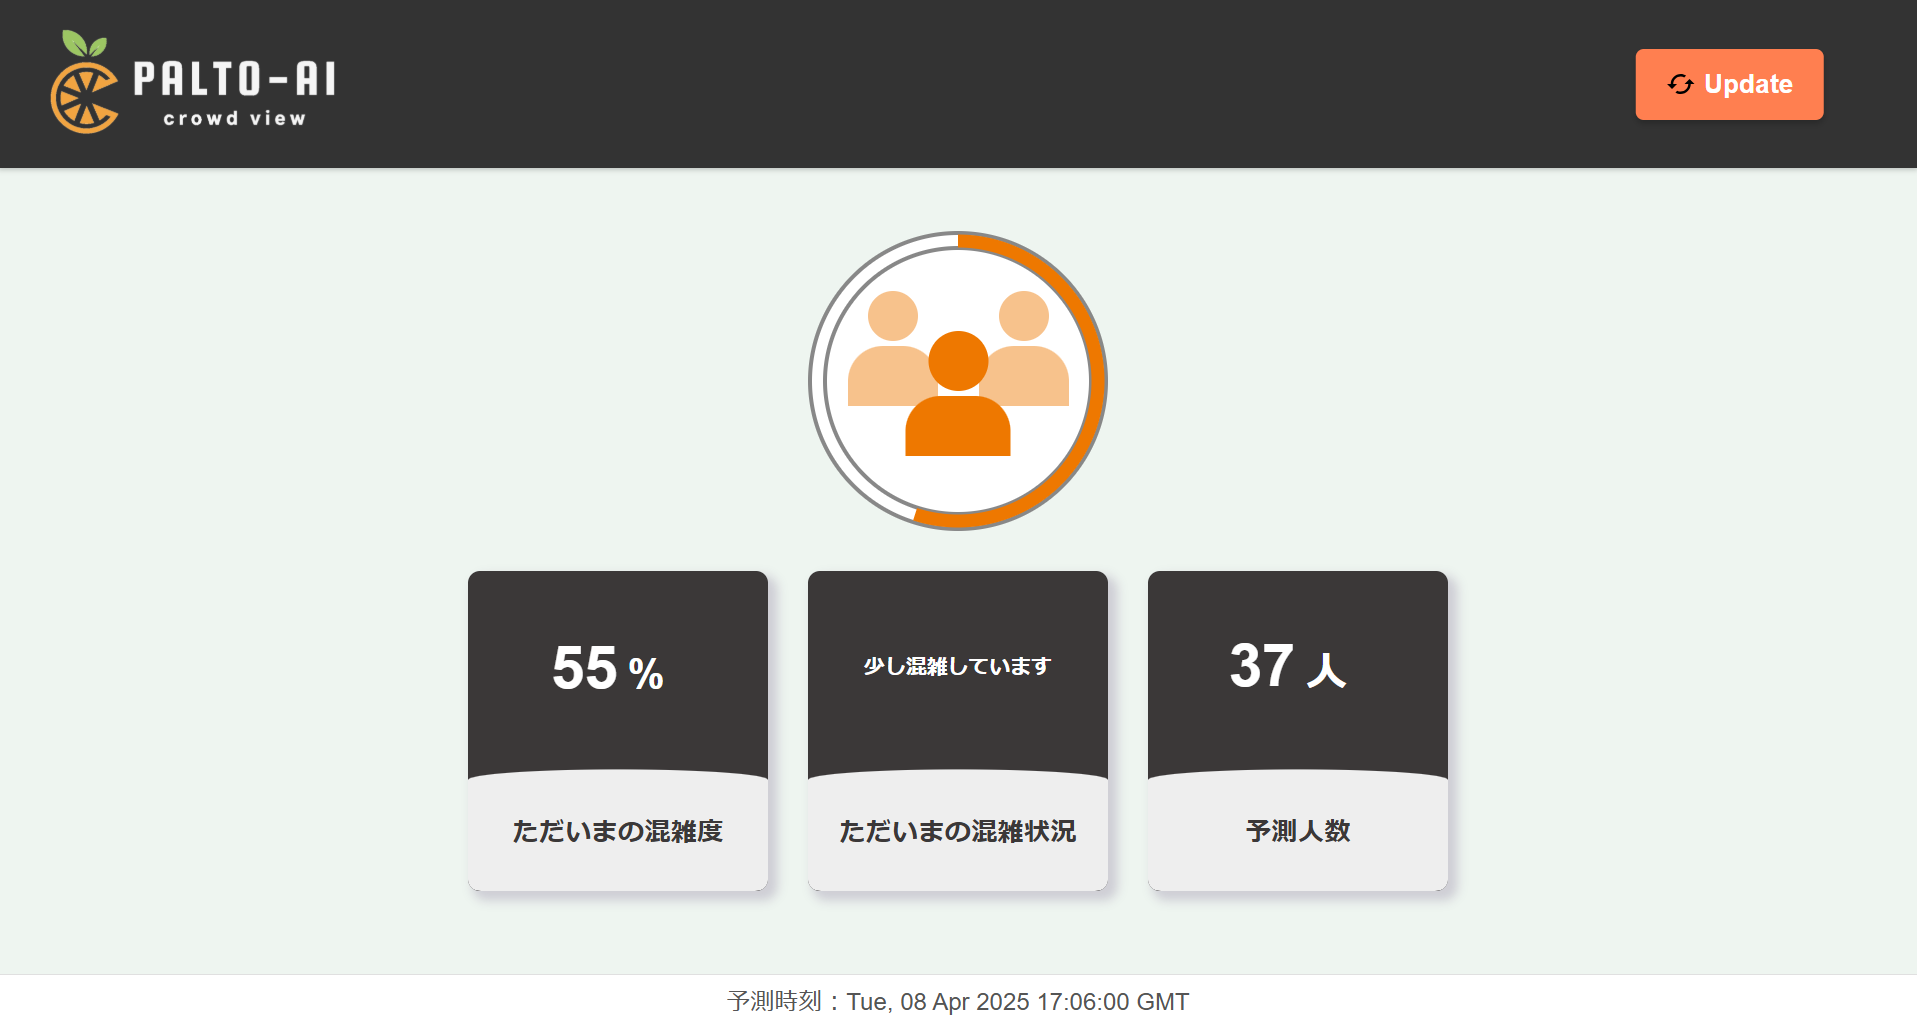
\includegraphics[width=1.0\linewidth]{images/webapp_screenshot.png}
	\caption{開発したWebアプリケーションの画面}
	\label{fig:webapp_screenshot}
\end{figure}

表\ref{tbl:UI_components}に,主要なUI要素とその役割,図\ref{fig:webapp_screenshot}に本システムのWebアプリケーション画面をそれぞれ示す.画面中央には混雑度を視覚的に表現するProgressRingコンポーネントを配置し,現在の混雑状況を円形プログレスバーと数値で直感的に把握できるようにしている.また,人物アイコン(GroupIcon)の色彩変化により,混雑度の程度を視覚的に表現している.

StatusBoxコンポーネントでは具体的な混雑状況の説明と予測人数を表示し,ユーザーに詳細情報を提供している.画面右上のUpdateButtonを押すことで,最新の予測データを取得できる仕組みとなっており,回転アニメーションによって更新中であることを示す視覚的フィードバックも実装している.

さらに,ResponsiveElementsの実装により,様々な画面サイズに対応したレイアウト調整が行われ,デスクトップからモバイルまで一貫したユーザーエクスペリエンスを提供している.これらのUI要素が連携することで,混雑状況を簡潔かつ分かりやすく伝えるインターフェースを実現した.